% !TEX root = ../../../../../temp_manuscript.tex

\epigraphhead[450]{\epigraph{\say{There are two things in life you can share to make people happy: love and data.}}{--- \textup{Fatih Incekara}}}
\chapter[The Erasmus Glioma Database (EGD): structural MRI scans, WHO 2016 subtypes, and segmentations of 774 patients with glioma][Erasmus Glioma Database]{The Erasmus Glioma Database (EGD): structural MRI scans, WHO 2016 subtypes, and segmentations of 774 patients with glioma}\label{chap:EGD}



\begin{ChapterAbstract}
The \gls{EGD} contains structural \gls{MRI} scans, genetic and histological features (specifying the \acrshort{WHO} 2016 subtype), and whole \gls{tumor} segmentations of patients with glioma.
Preoperative \gls{MRI} data of 774 patients with glioma (281 female, 492 male, 1 unknown, age range 19--86 years) treated at the Erasmus MC between 2008 and 2018 is available.
For all patients a pre-contrast \acrlong{T1}, \acrlong{T1C}, \acrlong{T2}, and \acrlong{T2} FLAIR scan are available, made on a variety of scanners from four different vendors.
All scans are registered to a common atlas and defaced.
Genetic and histological data consists of the \acrshort{IDH} mutation status (available for 467 patients), 1p/19q co-deletion status (available for 259 patients), and grade (available for 716 patients).
The full \acrshort{WHO} 2016 subtype is available for 415 patients.
Manual segmentations are available for 374 patients and automatically generated segmentations are available for 400 patients.
The dataset can be used to relate the visual appearance of the \gls{tumor} on the scan with the genetic and histological features, and to develop automatic segmentation methods.
\publishedas{voortunpublisedEGD}
\end{ChapterAbstract}

\begin{table}[htbp]
\begin{tabular}{L{4cm}C{0.2cm}L{8cm}}
\toprule
\textbf{Subject} && Medical imaging, clinical genetics\\
\\
\textbf{Specific subject area}  && Structural \acrshort{MRI} scans, \acrshort{WHO} 2016 subtypes, \gls{tumor} segmentations of patients with glioma.\\
\\
\textbf{Type of data}  && \acrshort{MRI} data (NIfTI files):\\
&& \hphantom{aaaaa}Pre-contrast \acrlong{T1}\\
&& \hphantom{aaaaa}\Acrlong{T1C}\\
&& \hphantom{aaaaa}\acrlong{T2}\\
&& \hphantom{aaaaa}\acrlong{T2} FLAIR\\
&& Genetic and histological data (Excel files):\\
&&\hphantom{aaaaa}\acrshort{IDH} mutation status\\
&&\hphantom{aaaaa}1p/19q co-deletion status\\
&&\hphantom{aaaaa}Grade\\
&&\Gls{tumor} segmentations (NIfTI files)\\
\\
\textbf{How data were acquired} && \acrshort{MRI} Scans were acquired on a variety of scanners and\\
&& field strengths from four different vendors.\\
&& Genetic and histological data were obtained by analysis of \gls{tumor} tissue obtained from biopsy or resection.\\
&& Whole \gls{tumor} segmentations were manually annotated by one of four different observers or automatically generated using a convolutional neural network \autocite{voortunpublishedsubtypingEGD}.\\
\\
\textbf{Description of data collection} && Patients with glioma treated at the Erasmus MC between 2008 and 2018 were retrospectively included.\\
&&Preoperative imaging was acquired according to routine clinical protocols.\\
&&\acrshort{IDH} mutation status, 1p/19q co-deletion status, and grade were determined either as part of the treatment process or for research purposes.\\
\\
\textbf{Data source location}  && Erasmus MC (University Medical Center Rotterdam),\\
&& Rotterdam, The Netherlands\\
\\
\textbf{Data accessibility}   && Repository name: Health-RI XNAT\\
                         &&Data identification number: EGD\\
                         &&Direct URL to data: \url{https://xnat.bmia.nl/data/archive/projects/egd}\\
\\
\textbf{Related research article} &&  S.R. van der Voort, F. Incekara, M.M.J. Wijnenga,\\
&&G. Kapsas, R. Gahrmann, J.W. Schouten, R. Nandoe Tewarie, G.J. Lycklama, P.C. De Witt Hamer, R.S. Eijgelaar, P.J. French, H.J. Dubbink, A.J.P.E. Vincent, W.J. Niessen, M.J. van den Bent, M. Smits, and S. Klein, \say{WHO 2016 subtyping and automated segmentation of glioma using multi-task deep learning}, \textit{submitted}\\
\bottomrule
\end{tabular}
\caption{Specifications of the data}\label{tab:egd_specifications}
\end{table}


\section{Value of the data}

\begin{itemize}
\itemsep=0pt
\parsep=0pt
\item This dataset provides imaging data, genetic and histological data, and outlined \glspl{tumor} from a large number of patients with glioma.
Currently, limited data is available that provides all this information for a single patient cohort.
Data has been collected from routine clinical care, thus representing the real-life variability of the data.
This real-life, heterogenous nature of the data, in combination with its size, makes the dataset a valuable resource.
\item This dataset will be beneficial for researchers working on the analysis of glioma based on \acrshort{MRI} scans.
\item This data can be used to validate or develop radiomics methods and automated segmentation methods.
For example, the data can be used as a large, heterogenous independent test set, or to increase the size and heterogeneity of train sets for developing new methods.
\end{itemize}


\section{Data description}

The \gls{EGD} contains 774 patients with glioma and provides three different sources of data:

\begin{enumerate}
  \item Structural \gls{MRI} scans
  \item Genetic and histological labels specifying the \gls{WHO} 2016 subtype
  \item \Gls{tumor} segmentations
\end{enumerate}

An overview of the data is presented in \cref{tab:egd_specifications}.
The data is available on an XNAT server which allows access to the data through an \acrshort{API} \autocite{marcus2007extensible}.
We have also created a Docker image that can be used to download the data locally according to the data structure described in this paper: \url{https://github.com/Svdvoort/egd-downloader}.

\subsection{Structural MRI scans}

For all patients four types of structural \gls{MRI} scans are available: pre-contrast \gls{T1}, \gls{T1C}, \gls{T2}, and \gls{FLAIR}\@.
These scans are provided as NIfTI files named \say{T1.nii.gz}, \say{T1GD.nii.gz}, \say{T2.nii.gz}, and \say{FLAIR.nii.gz}, with one folder per subject containing all four scans.
Scans have been converted from DICOM to NIfTI using dcm2niix version v1.0.20190410 \autocite{li2016first}, and have been registered to the MNI atlas using Elastix version 5.0.0 \autocite{shamonin2014fast,klein2010elastix}.
An overview of the \gls{MRI} vendor (DICOM tag (0008, 0070)), scanner model (DICOM tag (0008,1090)), and field strength (DICOM tag (0018,0087)) per patient is provided in the accompanying excel sheet \say{Scan\_characteristics.xlsx}.

Clinical data is provided in the Excel sheet \say{Clinical\_data.xlsx}, which includes the patient age in years at the time of the scan and the patient sex.
When the patient age or sex is unknown this is indicated by the label -1.


\subsection{Genetic and histological labels}
Genetic labels consist of the \gls{IDH} mutation status and the 1p/19q co-deletion status; histological labels consist of the \gls{tumor} grade.
These genetic and histological labels allow for the specification of the \gls{WHO} 2016 subtype \autocite{louis20162016}.
\gls{IDH} mutation status is available for 467 patients, 1p/19q co-deletion data is available for 259 patients, and \gls{tumor} grade is available for 716 patients; a detailed overview is given in \cref{fig:egd_venn_histo}.
For 222 patients the \gls{IDH} mutation status, 1p/19q co-deletion status, and \gls{tumor} grade are all known.
For 193 patients the \gls{IDH} mutation status and grade are known where the \gls{tumor} was either \gls{IDH}-wildtype or was a grade IV \gls{tumor}, obviating the need for the 1p/19q co-deletion status to determine the \gls{WHO} 2016 subtype.
Thus, the full \gls{WHO} 2016 subtype is available for 415 patients.

The genetic and histological labels for each patient are available as an Excel sheet: \say{Genetic\_and\_Histological\_labels.xlsx}.
For the \gls{IDH} mutation status and the 1p/19q co-deletion status patients have either label 1 (when the \gls{tumor} was \gls{IDH}-mutated or 1p/19q co-deleted, respectively) or label 0 (when the \gls{tumor} was \gls{IDH}-wildtype or 1p/19q intact, respectively).
Grade is indicated with label 2, 3, or 4 for \gls{WHO} grade II, III, or IV, respectively.
For all cases missing data is indicated by the label -1.

\begin{figure}
  \centering
  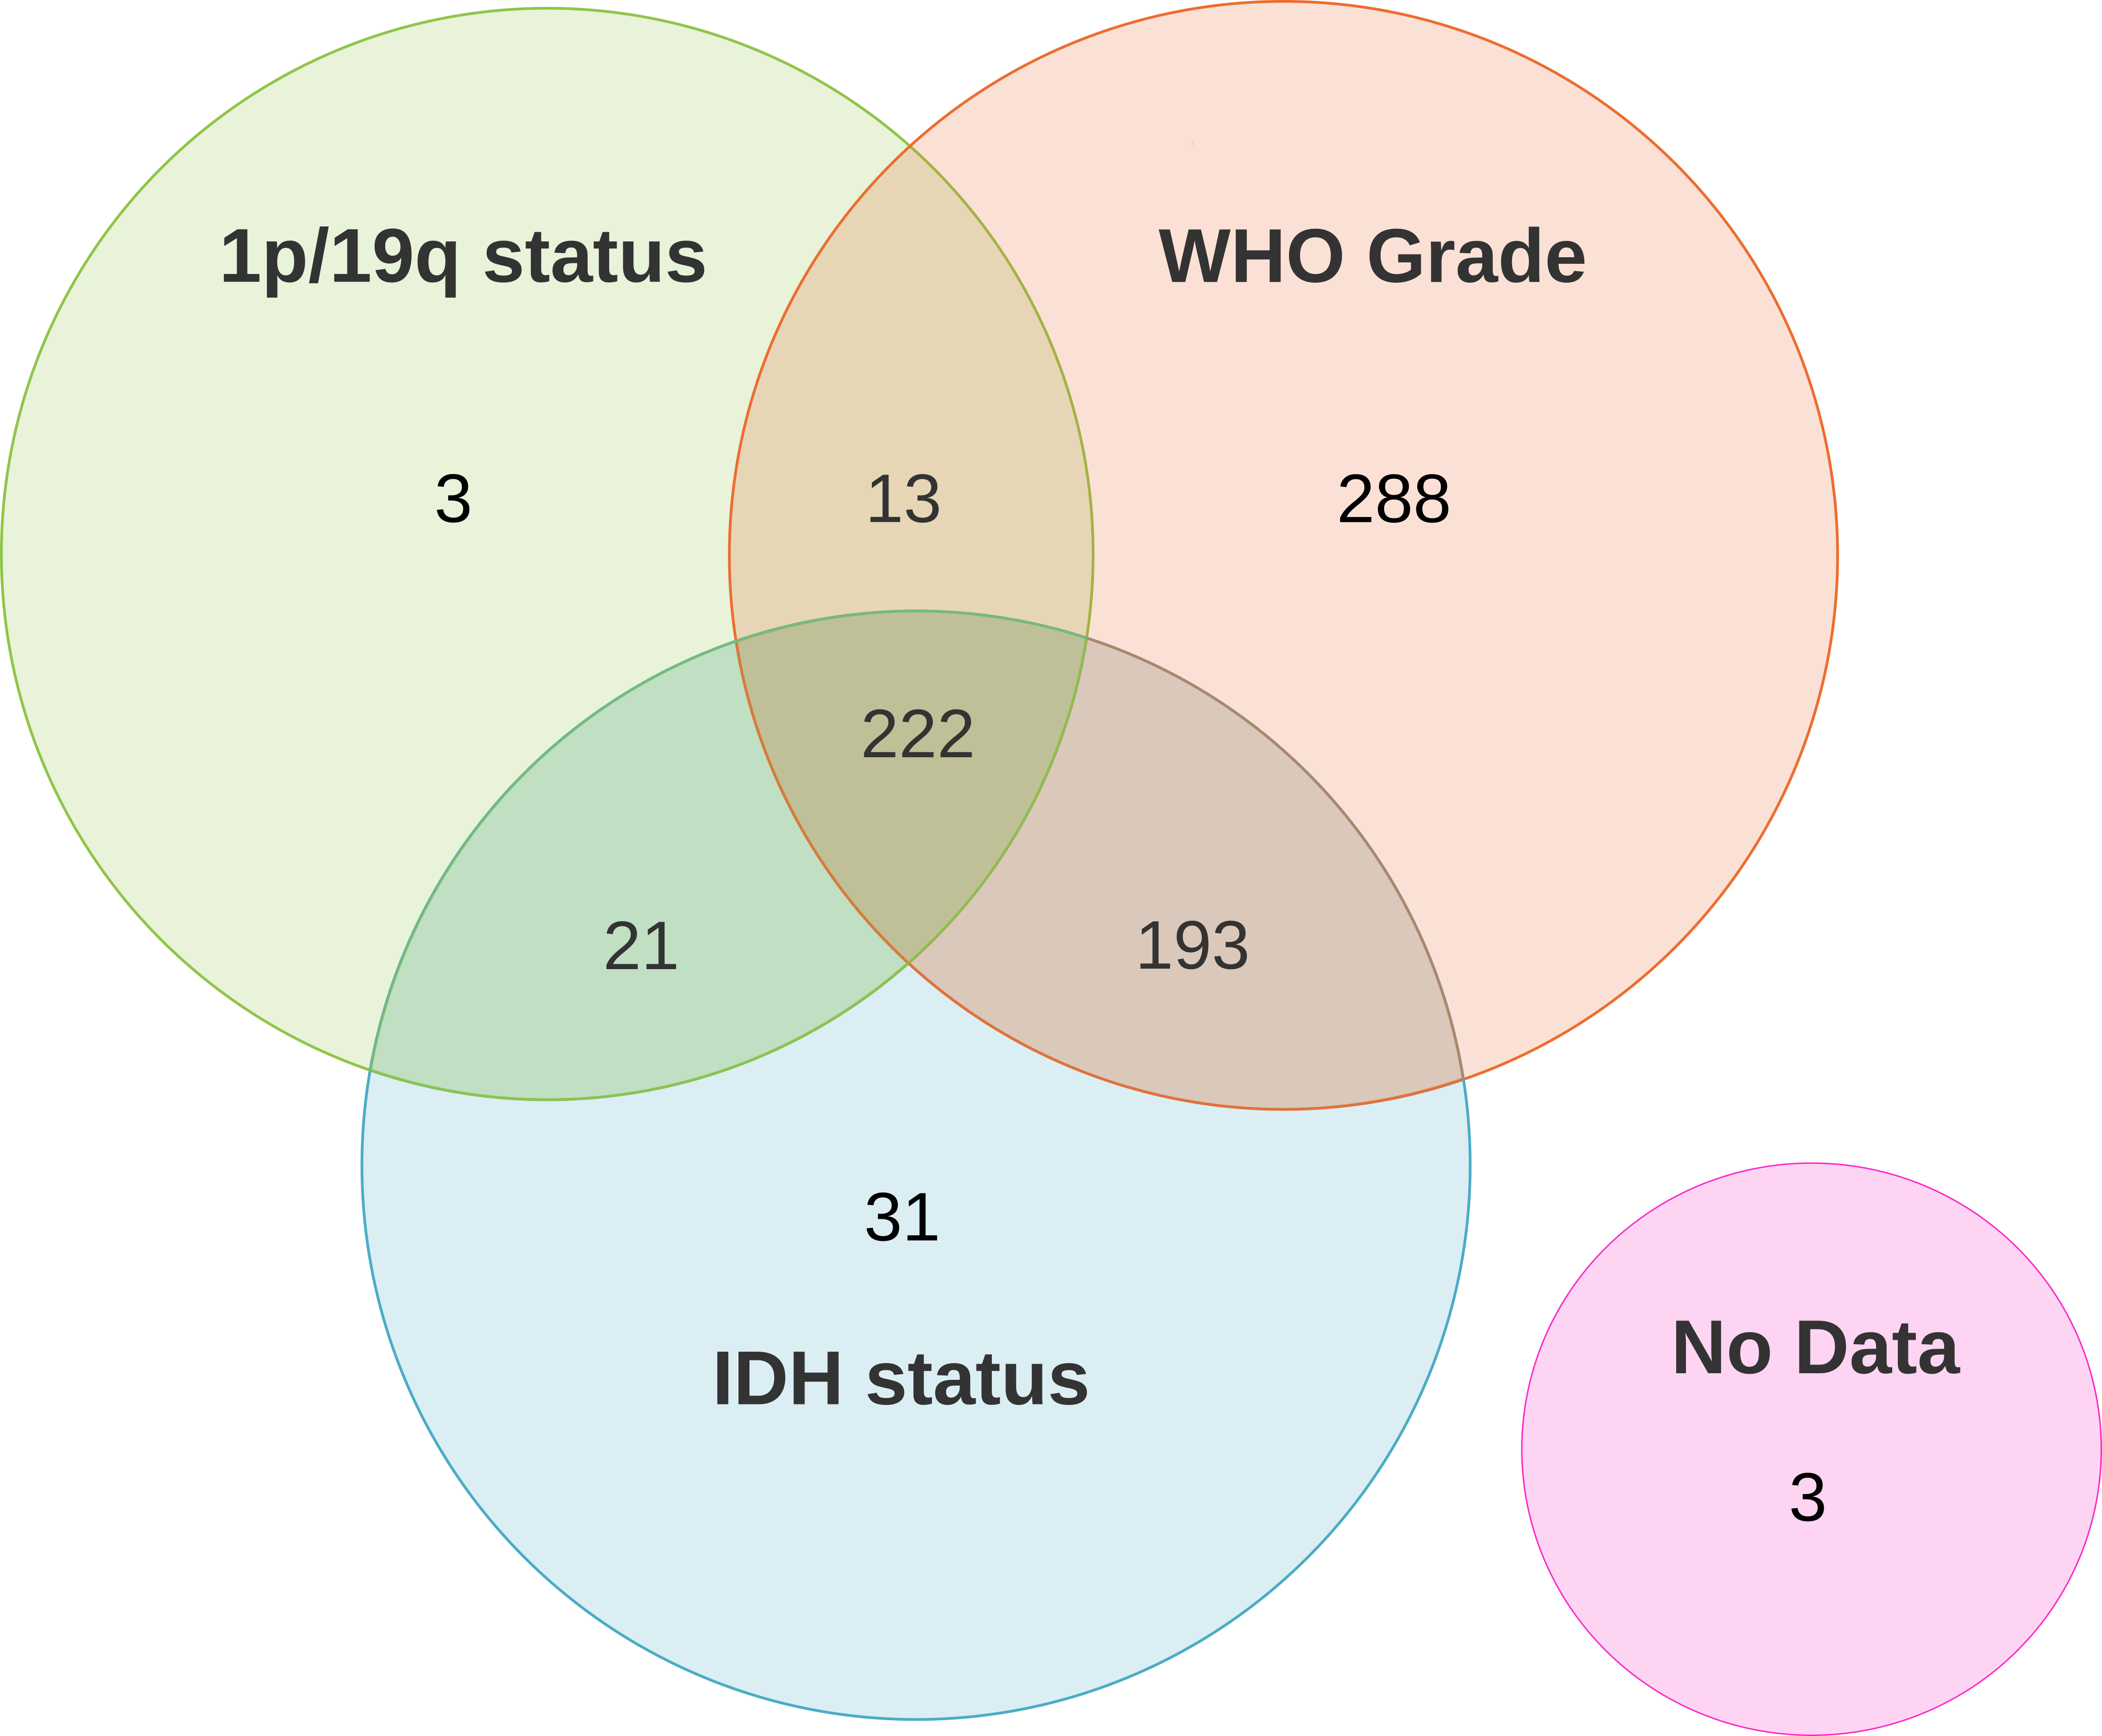
\includegraphics[width=0.65\textwidth]{Figures/venn_diagram_genetic_and_histological.png}
  \caption{Overview of number of patients with available genetic and histological data and the overlap between different groups.
  The \acrshort{WHO} 2016 subtype is available for the 222 patients for which the \acrshort{IDH} mutation status, 1p/19q co-deletion status, and \gls{tumor} grade is known and for the 193 patients for which the \acrshort{IDH} mutation status and \gls{tumor} grade is known}\label{fig:egd_venn_histo}
\end{figure}

\subsection{\Gls{tumor} segmentations}
For 374 patients a manually annotated whole \gls{tumor} segmentation and for 400 patients an automatic whole \gls{tumor} segmentation is available as \say{MASK.nii.gz} in the patient subfolder, alongside the four scans.
A label of 1 indicates \gls{tumor}, and a label of 0 indicates background.
The manual \gls{tumor} segmentations were made by one of four different observers based on either the \gls{T2} scan or the \gls{FLAIR} scan.
The automatic \gls{tumor} segmentations were made based on the  \gls{T1} scan, the \gls{T1C} scan, the \gls{T2} scan, and the \gls{FLAIR} scan using a \gls{CNN} \autocite{voortunpublishedsubtypingEGD}.
This \gls{CNN} was trained using the manually segmented scans (in addition to other manually segmented scans not included in this data release), therefore, the \gls{CNN} was not used to create automatic segmentations for the manually segmented scans.
The Excel sheet \say{Segmentation\_source.xlsx} provides an overview of the observer of the segmentation, indicated as OBS1, OBS2, OBS3, or OBS4 for the four manual observers or as AUTO if the segmentation was made by the \gls{CNN}.
The scan that was used as the basis of the segmentation for the manually annotated scans is also specified in this Excel sheet.

The data that is available in the Excel sheets (the scanner data, clinical data, genetic and histological labels, and information about the segmentation) is also available in each patient folder as \say{metadata.json} to allow for easier automatic processing.

\section{Experimental design, materials and methods}

Data was retrospectively collected for patients with diffuse glioma who were treated at the Erasmus MC, The Netherlands, between 2008 and 2018.
Patients were included if they were at least 18 years old and if preoperative \gls{T1}, \gls{T1C}, \gls{T2}, and \gls{FLAIR} were available.

\subsection{Imaging}

Scans were retrospectively collected from the imaging that was performed as part of the routine clinical care for each patient.
Scans were acquired on scanners from four vendors: Siemens (347 patients), Philips (254 patients), GE (172 patients), and Toshiba (1 patient), using a field strength of \SI{3}{\tesla} (83 patients), \SI{1.5}{\tesla} (571 patients), \SI{1}{\tesla} (110 patients), or \SI{0.5}{\tesla} (6 patients).
For 4 patients the field strength was not known.

All scans were registered to the MNI152 atlas, version ICBM 2009a nonlinear symmetric, which has a voxel size of $1 \times 1 \times 1$ \si{\cubic\milli\metre} and a size of $197 \times 233 \times 189$ voxels \autocite{fonov2009unbiased,fonov2011unbiased}.
The scans were affinely registered using Elastix version 5.0.0 \autocite{shamonin2014fast,klein2010elastix}.
The pre- and post-contrast \gls{T1} scans were registered to the \gls{T1} atlas; the \gls{T2} and \gls{FLAIR} scans were registered to the \gls{T2} atlas.
When a manual segmentation was available for a patient, the registration parameters that resulted from registering the scan used during the segmentation were used to transform the segmentation to the atlas.
Registration parameters are available at the Elastix Model Zoo  under ID Par0064 (\url{https://elastix.lumc.nl/modelzoo/par0064/}).

After image registration, the scans were then defaced using a mask that was created based on the MNI atlas; this mask is available as \say{Deface\_mask.nii.gz}.
All voxels outside this mask were set to 0, voxels within the mask kept their original value.
The defacing mask included as much of the skull as possible, while ensuring the privacy of the patient by removing the characteristic facial features.
For future processing of the dataset a brain mask that can be used for skull stripping is also included, available as \say{Brain\_mask.nii.gz}.
This brain mask was made using HD-BET \autocite{isensee2019hdbet}.

\subsection{Genetics}

Genetic and histological features were determined from \gls{tumor} tissue that was obtained through biopsy or resection as part of the routine clinical care.
\Gls{FFPE} tissue sections were macro-dissected, selected for areas with highest \gls{tumor} content as marked by the neuro-pathologist.
DNA was isolated from these sections as described by \citeauthorref{wijnenga2018prognostic}.
A dedicated sequencing panel was then used for the molecular analysis to screen for \gls{IDH}1 or \gls{IDH}2 mutations and 1p/19q co-deletion \autocite{dubbink2015molecular}.

\subsection{Segmentation}
Manual segmentations were made using SimpleITK v3.6.0 \autocite{yushkevich2006user} or BrainLab (BrainLab, Feldkirchen, Germany, version 2.1.0.15), with which the whole \gls{tumor} was segmented based on the hyperintensities on either the \gls{T2} scan or the \gls{FLAIR} scan.
Manual segmentations were made based on the scans before registration to the atlas.

Automatic segmentations were based on the registered scans, and were generated using a \gls{CNN}; for more details see \citeauthorref{voortunpublishedsubtypingEGD}.

\section*{Ethics Statement}
The study was performed in accordance with the 1964 Helsinki Declaration and its later amendments or comparable ethical standards.


\section*{Acknowledgments}
Sebastian van der Voort and Fatih Incekara acknowledge funding by the Dutch Cancer Society (KWF project number EMCR 2015-7859).

